% A pure minimalistic LaTeX-Beamer theme for everyone to use.
% Copyright (C) 2020 Kai Norman Clasen
% Edited by Lucas Saldyt

\documentclass[aspectratio=169]{beamer}
\DeclareMathSizes{12}{30}{16}{12}
% should also look nice for the classic aspectratio
% of course, than the text has to be refitted
% \documentclass{beamer} 
\usepackage[utf8]{inputenc}
\usepackage[T1]{fontenc}
\usepackage{tikz}
\usepackage{amsmath}
\usepackage[export]{adjustbox}

\DeclareMathOperator*{\argmin}{\arg\!\min}
\DeclareMathOperator*{\argmax}{\arg\!\max}

% \usetheme[nofooter, darkmode]{pureminimalistic}
% \usetheme[nofooter]{pureminimalistic}
% \usetheme[nofooter]{pureminimalistic}
\usetheme[showmaxslides, darkmode]{pureminimalistic}

% \usepackage[backend=biber,style=apa,autocite=inline]{biblatex}
% \usepackage[american]{babel}
\usepackage[american]{babel}
\usepackage{csquotes}
\usepackage[style=apa, backend=biber]{biblatex}
\DeclareLanguageMapping{american}{american-UoN}

% \usepackage[english]{babel}
% \usepackage[backend=biber,style=apa]{biblatex}
% \DeclareLanguageMapping{english}{english-apa}
\addbibresource{sources.bib}

% this makes it possible to add backup slides, without counting them
\usepackage{appendixnumberbeamer}
\renewcommand{\appendixname}{\texorpdfstring{\translate{appendix}}{appendix}}

\renewcommand{\logotitle}{
\includegraphics[width=.2\linewidth]{logos/asu_logo_alt.png}}
\renewcommand{\logoheader}{}
\renewcommand{\logofooter}{
\includegraphics[width=.15\linewidth]{logos/asu_logo_alt.png}}

\definecolor{m1}{RGB}{30, 76, 214}
\definecolor{m2}{RGB}{161, 3, 74}
\definecolor{m3}{RGB}{255, 132, 0}
\definecolor{m4}{RGB}{255, 196, 0}
\definecolor{m5}{RGB}{3, 171, 34}
\definecolor{grey}{RGB}{130, 130, 130}

% if loaded after begin{document} a warning will appear: "pdfauthor already used"
\title[Learning Diverse Programs]{Lifelong Learning for Path-Planning via Genetic Programming}
\author{Lucas Saldyt}
\institute{Arizona State University} 
\date{\today}

\begin{document}
% has to be loaded outside of a frame to work!
\maketitle

\begin{frame}[plain]
  % This is a robot.
  % This particular robot was designed for mars.
  % This design was done by hand, with high reliability in mind
  \begin{figure}
  \centering
  \vspace*{-1em}
  \hspace*{-3em}
  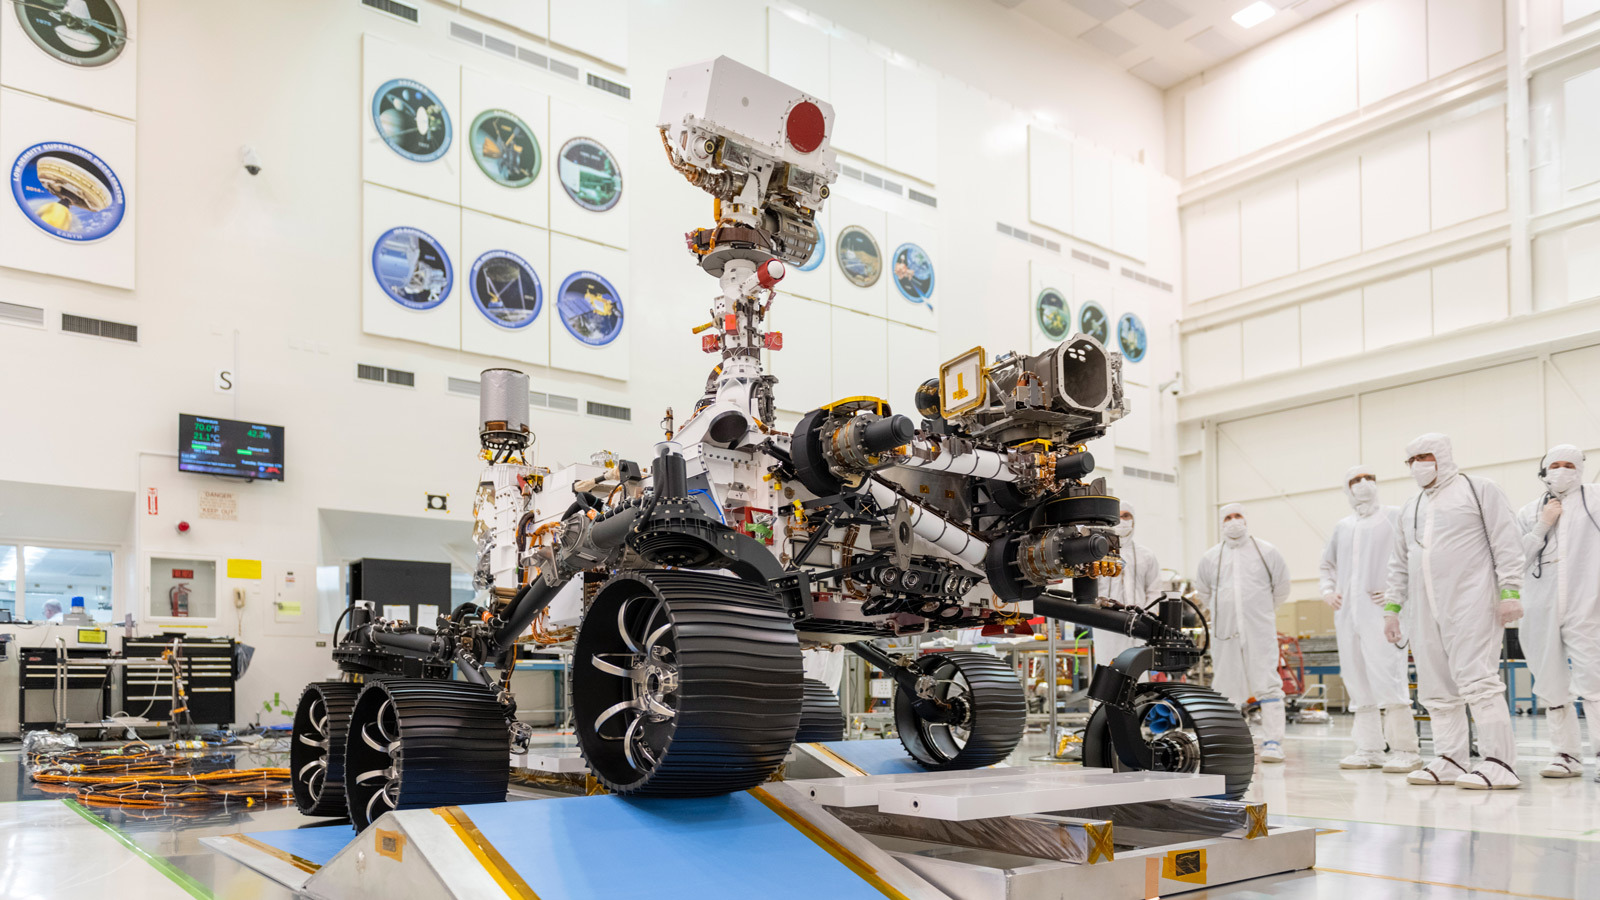
\includegraphics[height=9.5cm,keepaspectratio]{figures/perseverance.jpg}
  \end{figure}
\end{frame}

\begin{frame}[plain]
  % This is the surface of mars
  % It represents a very unique environment
  
  \begin{figure}
  \centering
  \vspace*{-1em}
  \hspace*{-3em}
  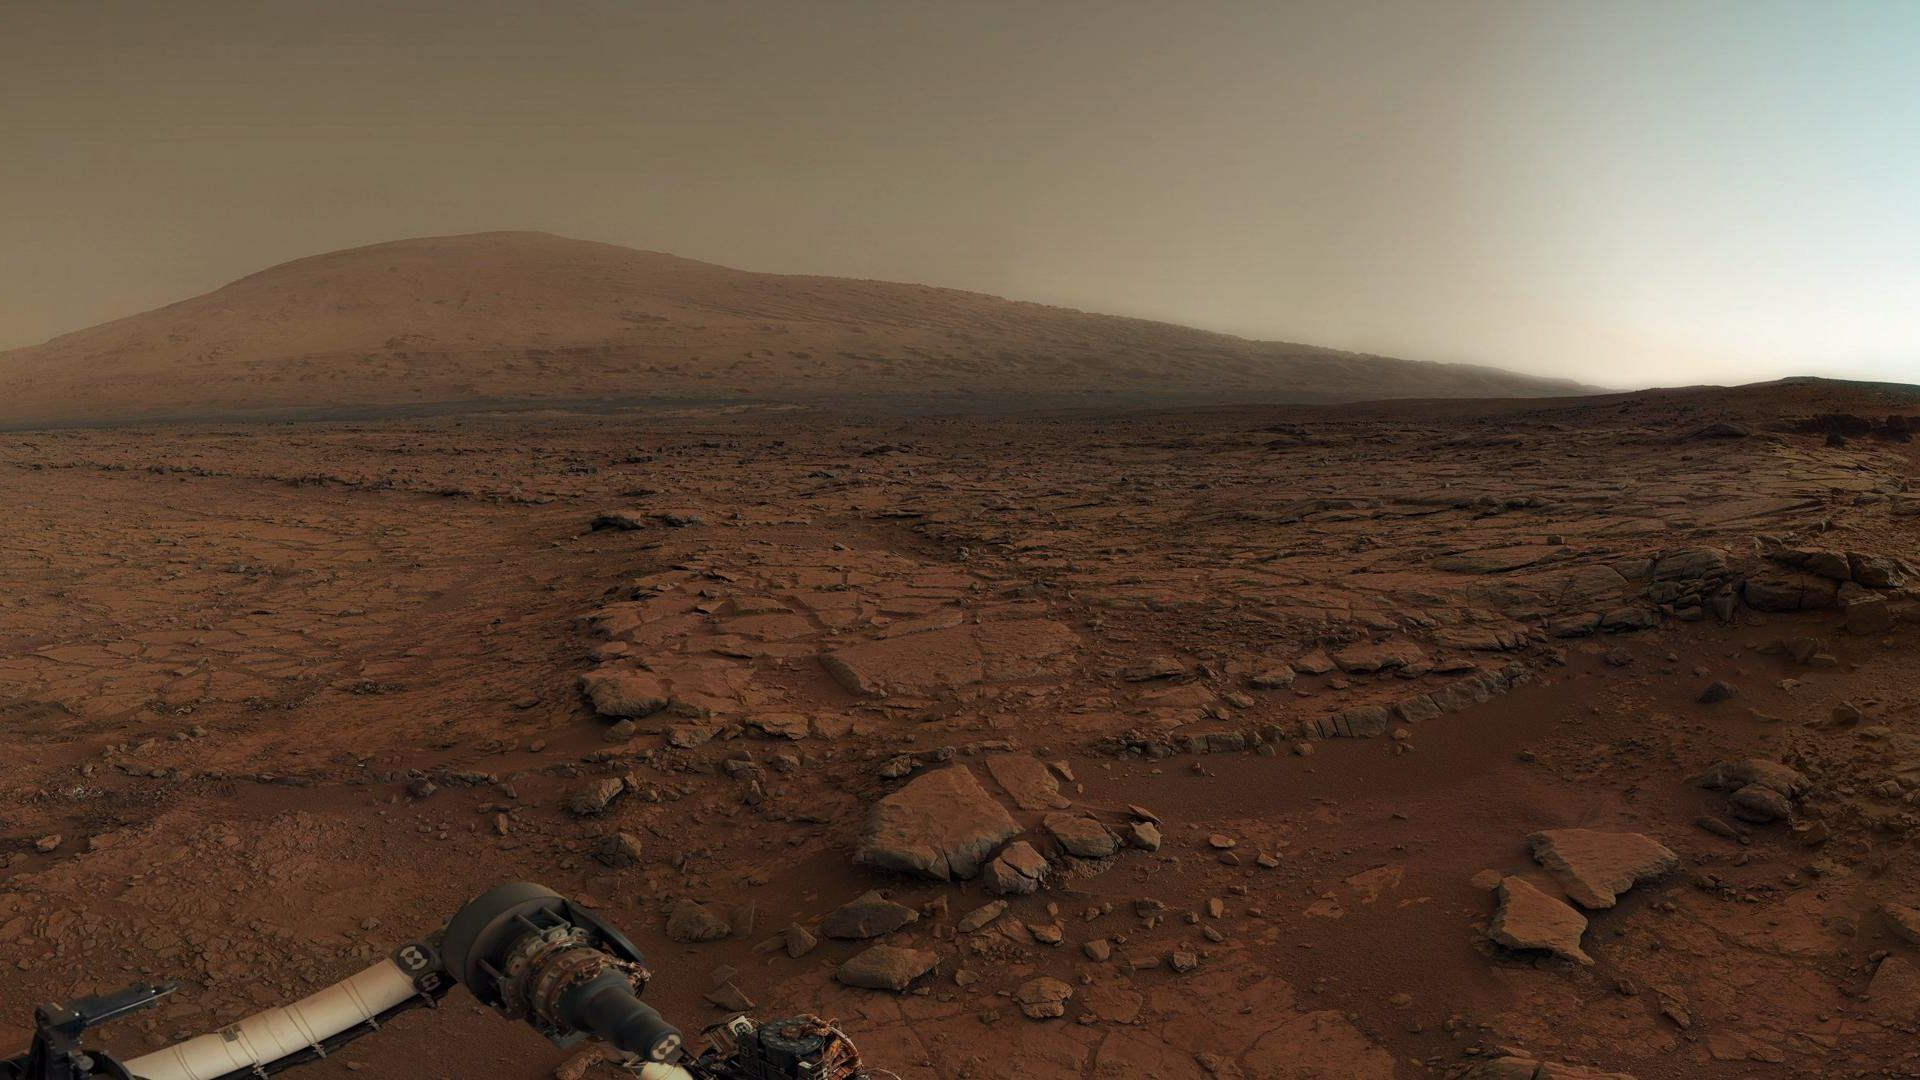
\includegraphics[height=9.5cm,keepaspectratio]{figures/mars_surface.jpg}
  \end{figure}
\end{frame}

\begin{frame}[plain]
  \begin{figure}
  \centering
  \vspace*{-1em}
  \hspace*{-3em}
  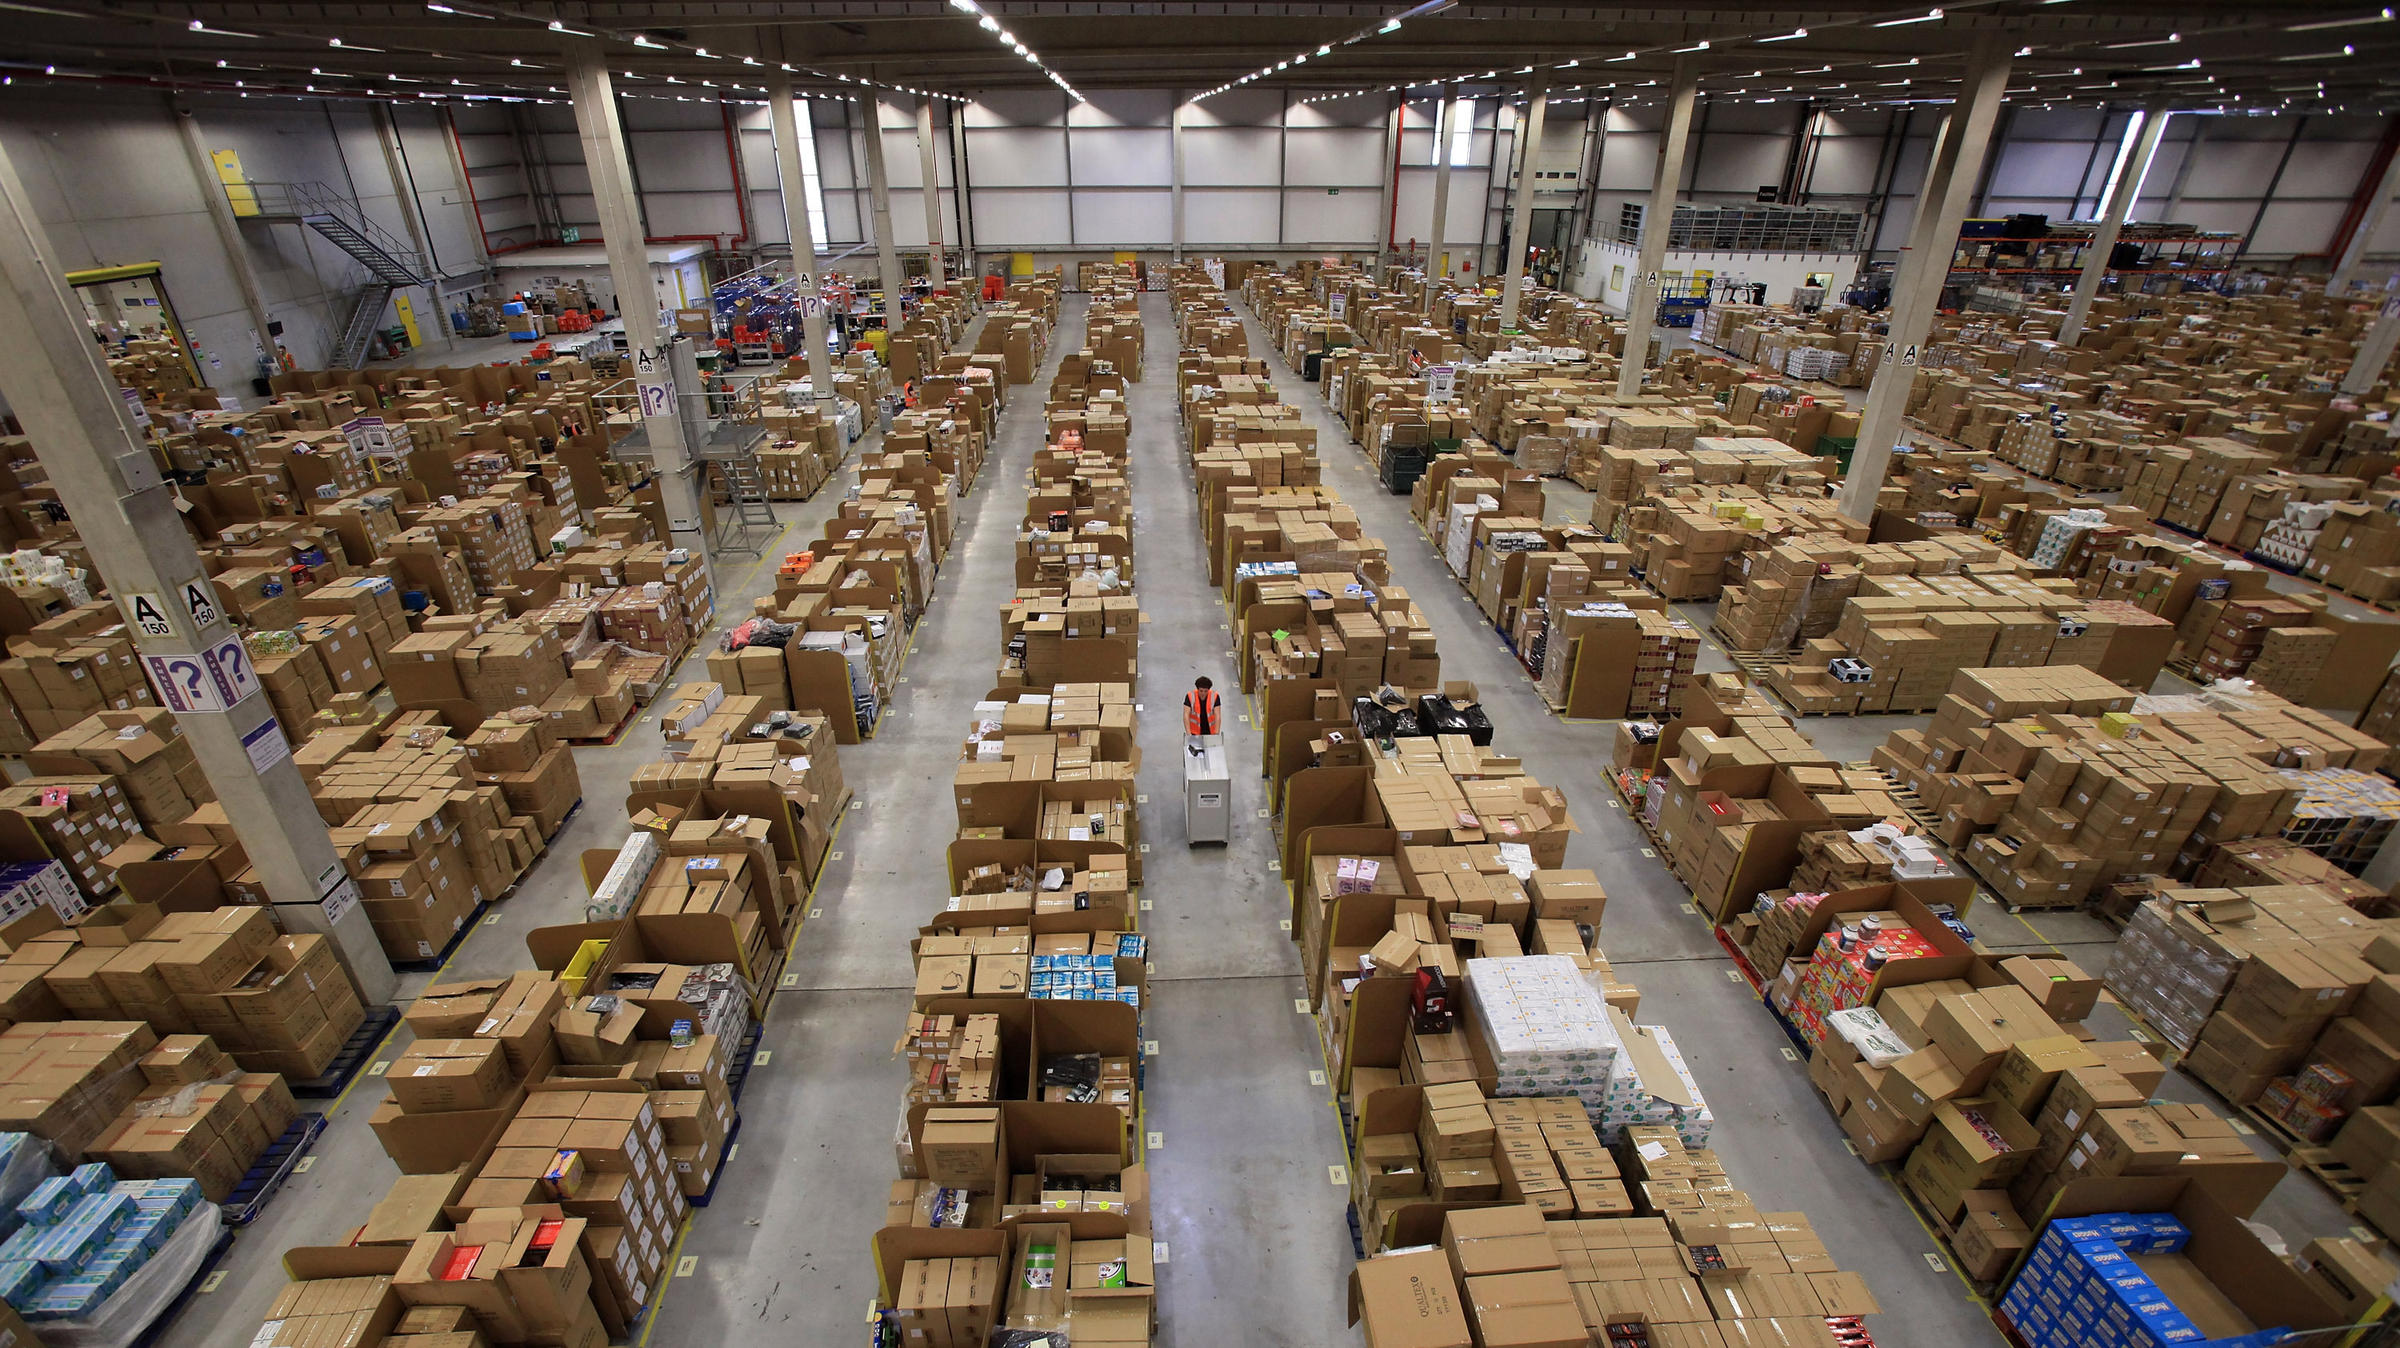
\includegraphics[height=9.5cm,keepaspectratio]{figures/warehouse.jpg}
  \end{figure}
\end{frame}

\begin{frame}[plain]{{\color{pureminimalistic@text@white} Core Goals \& Concepts}}
  \begin{columns}[T]
      \begin{column}{.6\linewidth}
          \begin{vfilleditems}
            \item {\Huge \color{pureminimalistic@text@red} Learning}
              \begin{itemize}
                \item {\Medium Flexibility}
              \end{itemize}
            \item {\Huge \color{pureminimalistic@text@red} Specialization}
              \begin{itemize}
                \item {\Medium Learn specific environment details?}
              \end{itemize}
            \item {\Huge \color{pureminimalistic@text@red} Generalization}
              \begin{itemize}
                \item {\Medium Learn general task proficiency?}
              \end{itemize}
            \item {\Huge \color{pureminimalistic@text@red} Curiosity}
              \begin{itemize}
                \item {\Medium Learn simply to explore efficiently?}
              \end{itemize}
          \end{vfilleditems}
      \end{column}
      \begin{column}{.4\linewidth}
          \begin{figure}
              \centering
              \caption{Where is this image from?}
              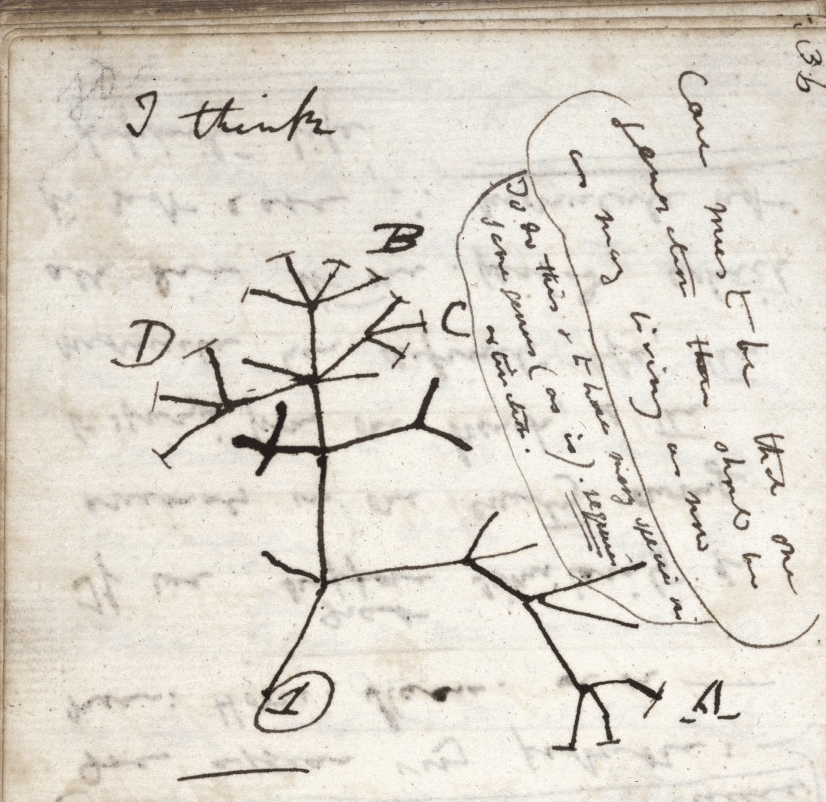
\includegraphics[height=5.5cm, keepaspectratio]{figures/i_think.png}
              \caption{"I think"}
              \label{fig:my_label}
          \end{figure}
      \end{column}
  \end{columns}
\end{frame}

\begin{frame}[plain]
  \begin{figure}
  \vspace*{-2em}
  \hspace*{-3em}
  \centering
  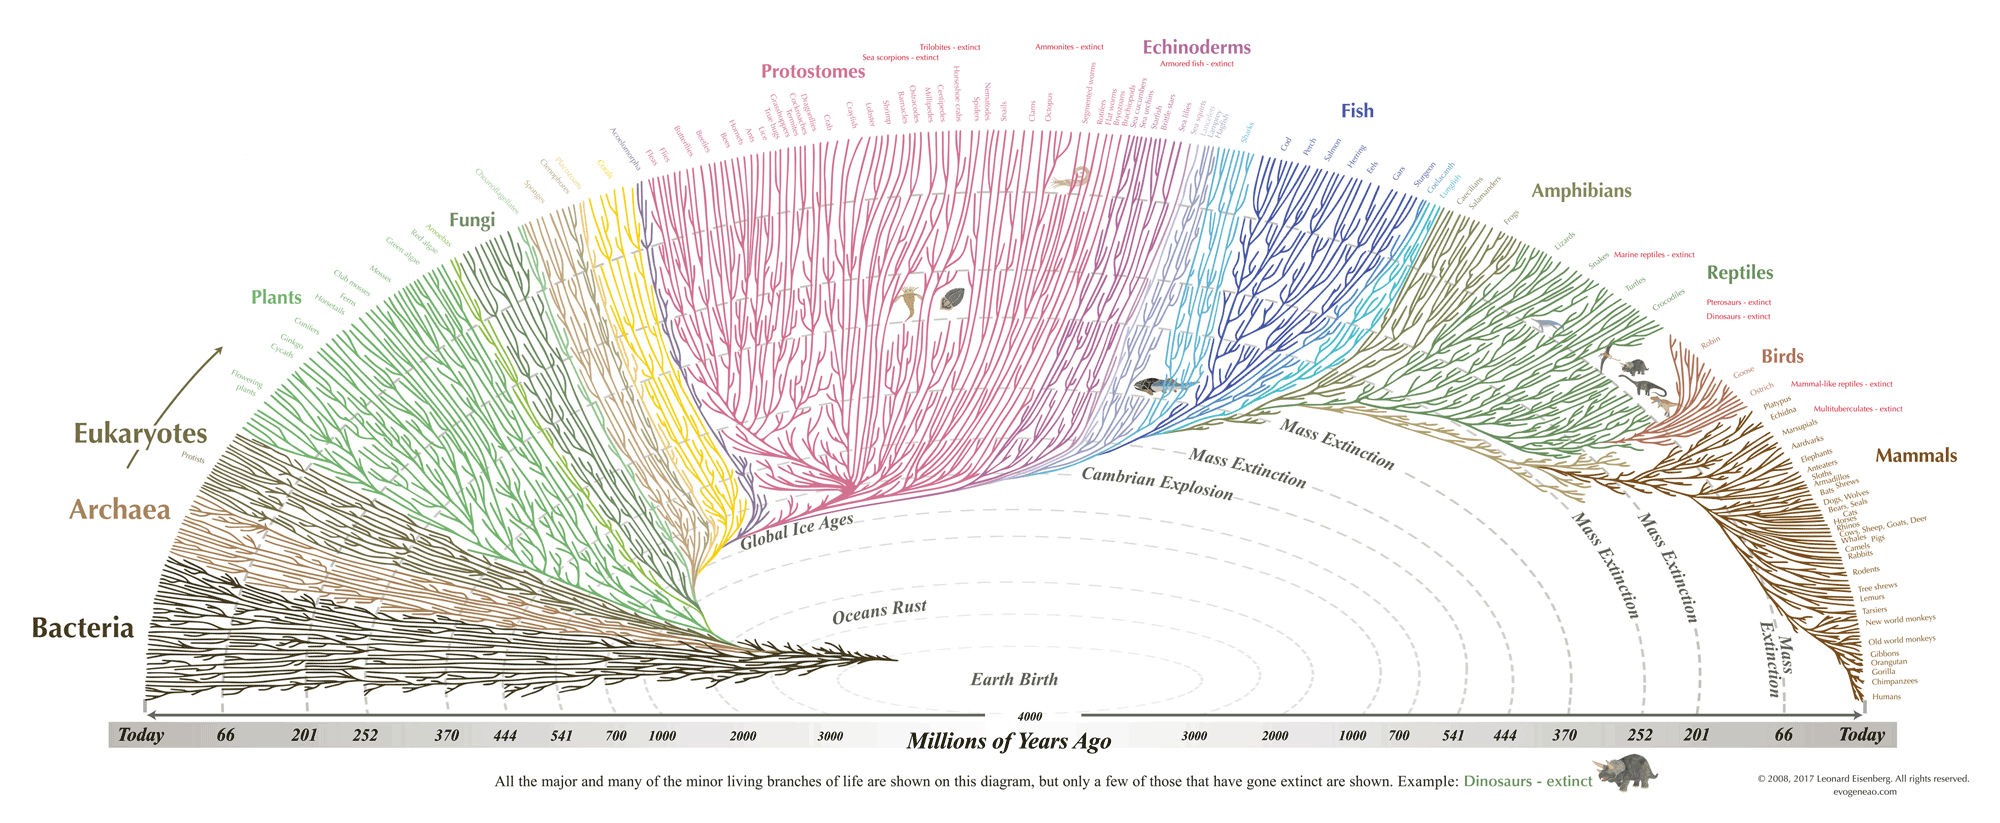
\includegraphics[width=1.17\linewidth,keepaspectratio]{figures/tree_of_life.png}
  \end{figure}
  {\color{pureminimalistic@text@red} \Huge Natural evolution}
\end{frame}

\begin{frame}[plain]
  \begin{figure}
  \centering
  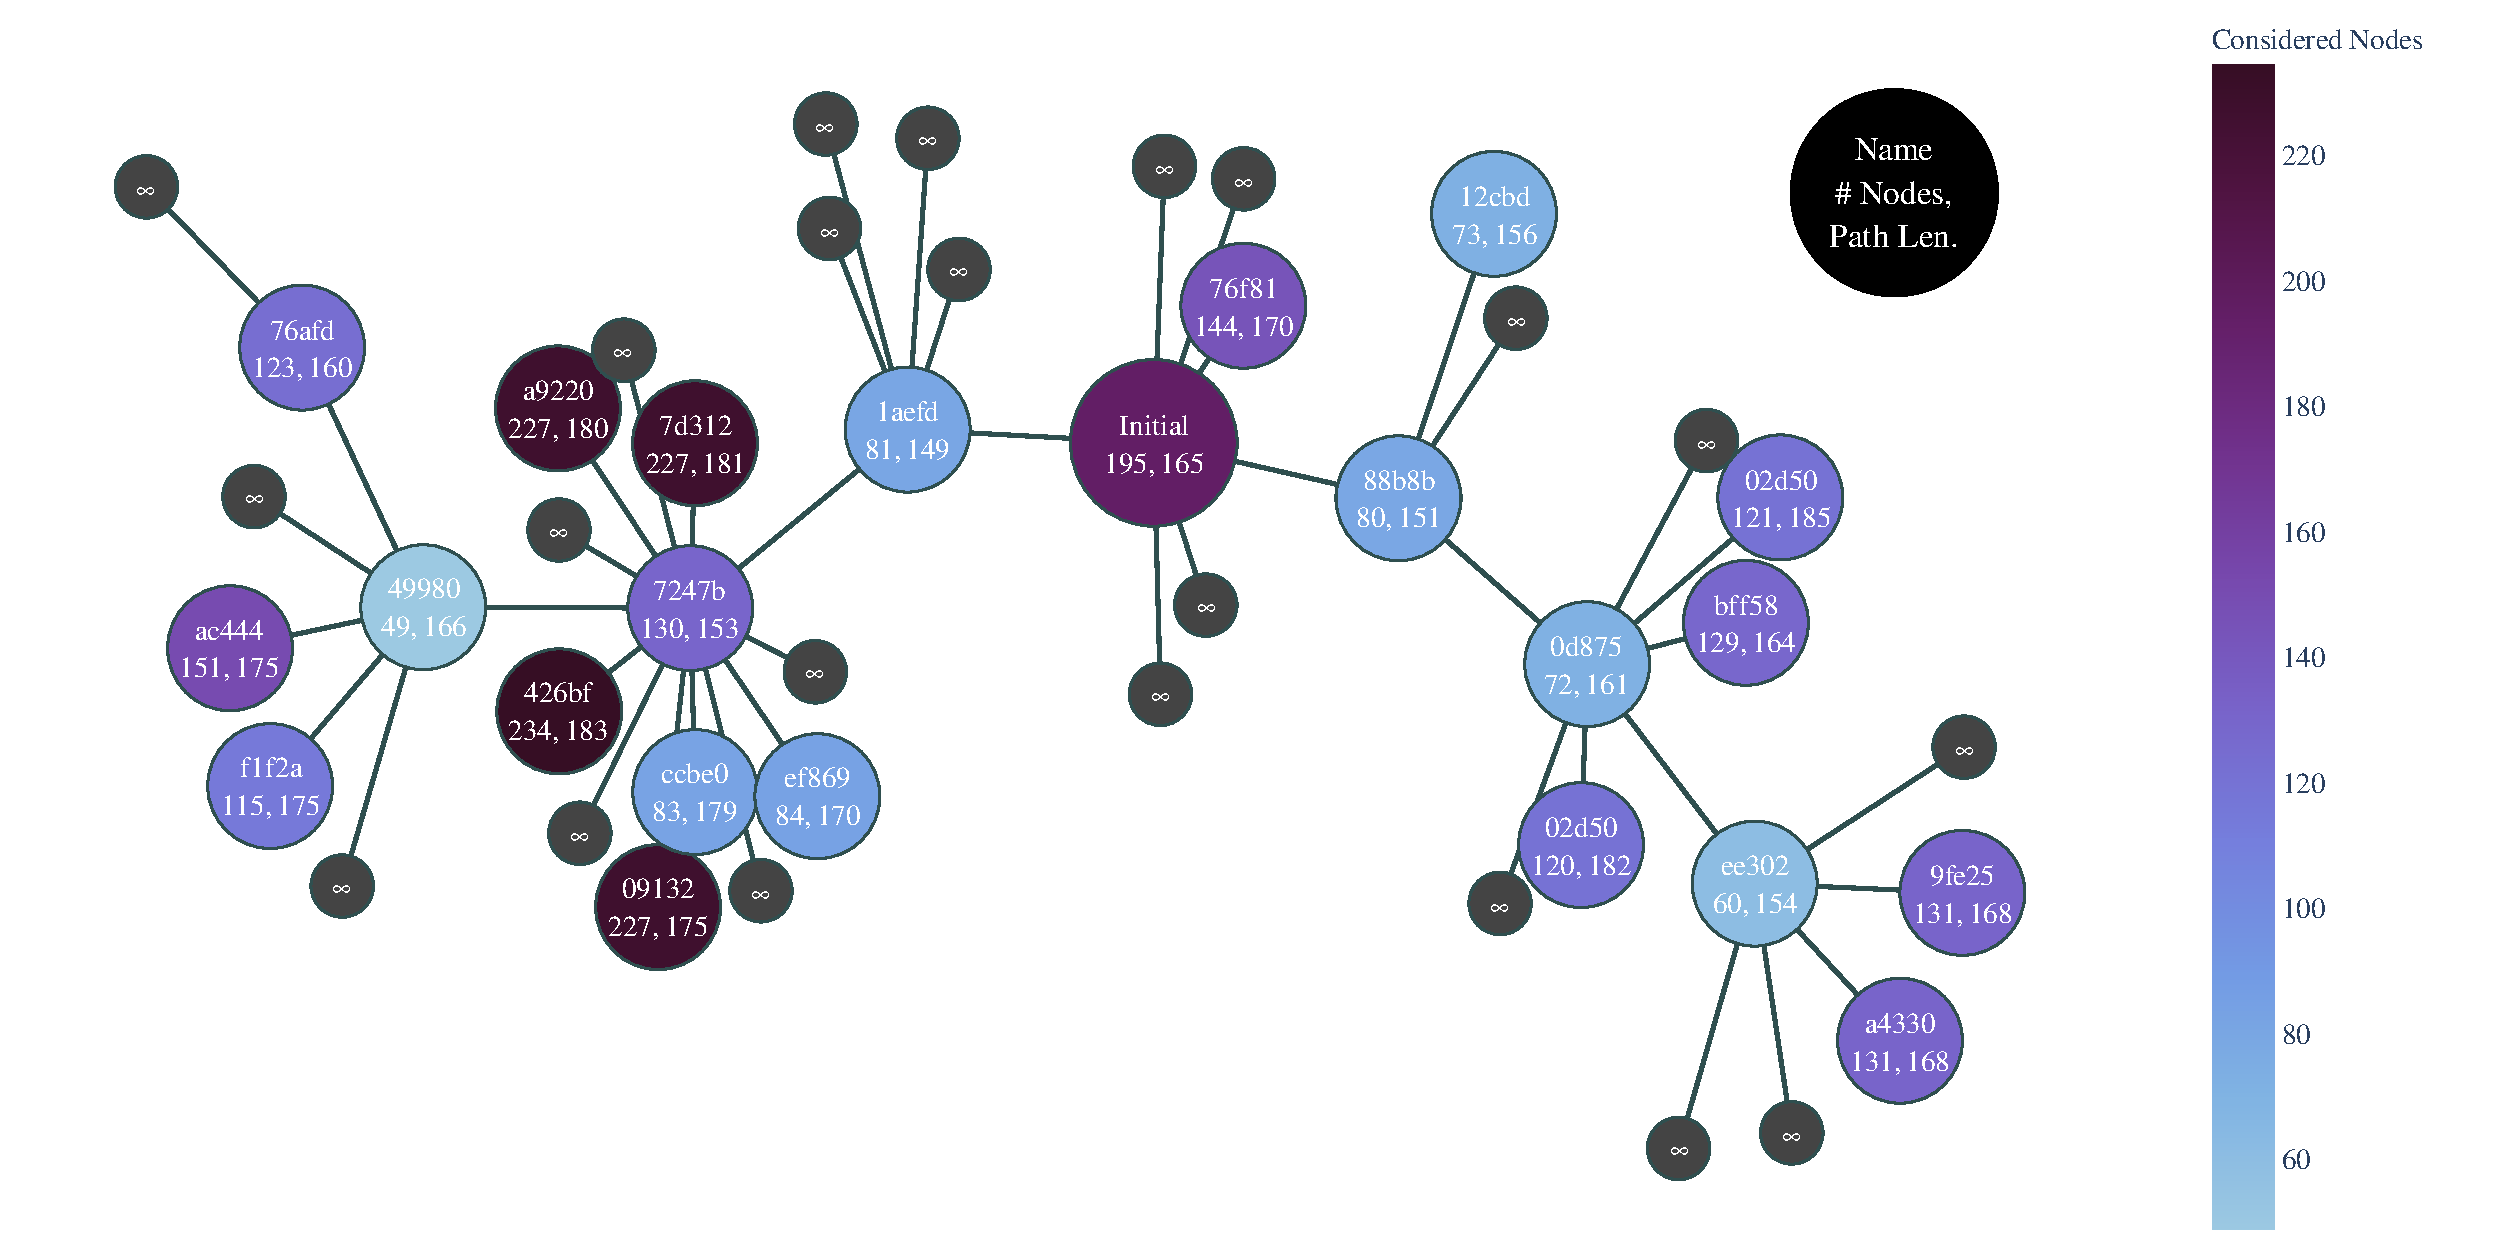
\includegraphics[width=1.0\linewidth,keepaspectratio]{figures/mutation_tree_starcraft_enigma_nsga2.pdf}
  \end{figure}
  {\color{pureminimalistic@text@red} \Huge Example Phylogenetic Tree}
\end{frame}

\begin{frame}[plain]{Problems Considered}
  \begin{columns}[T]
      \begin{column}{.5\linewidth}
          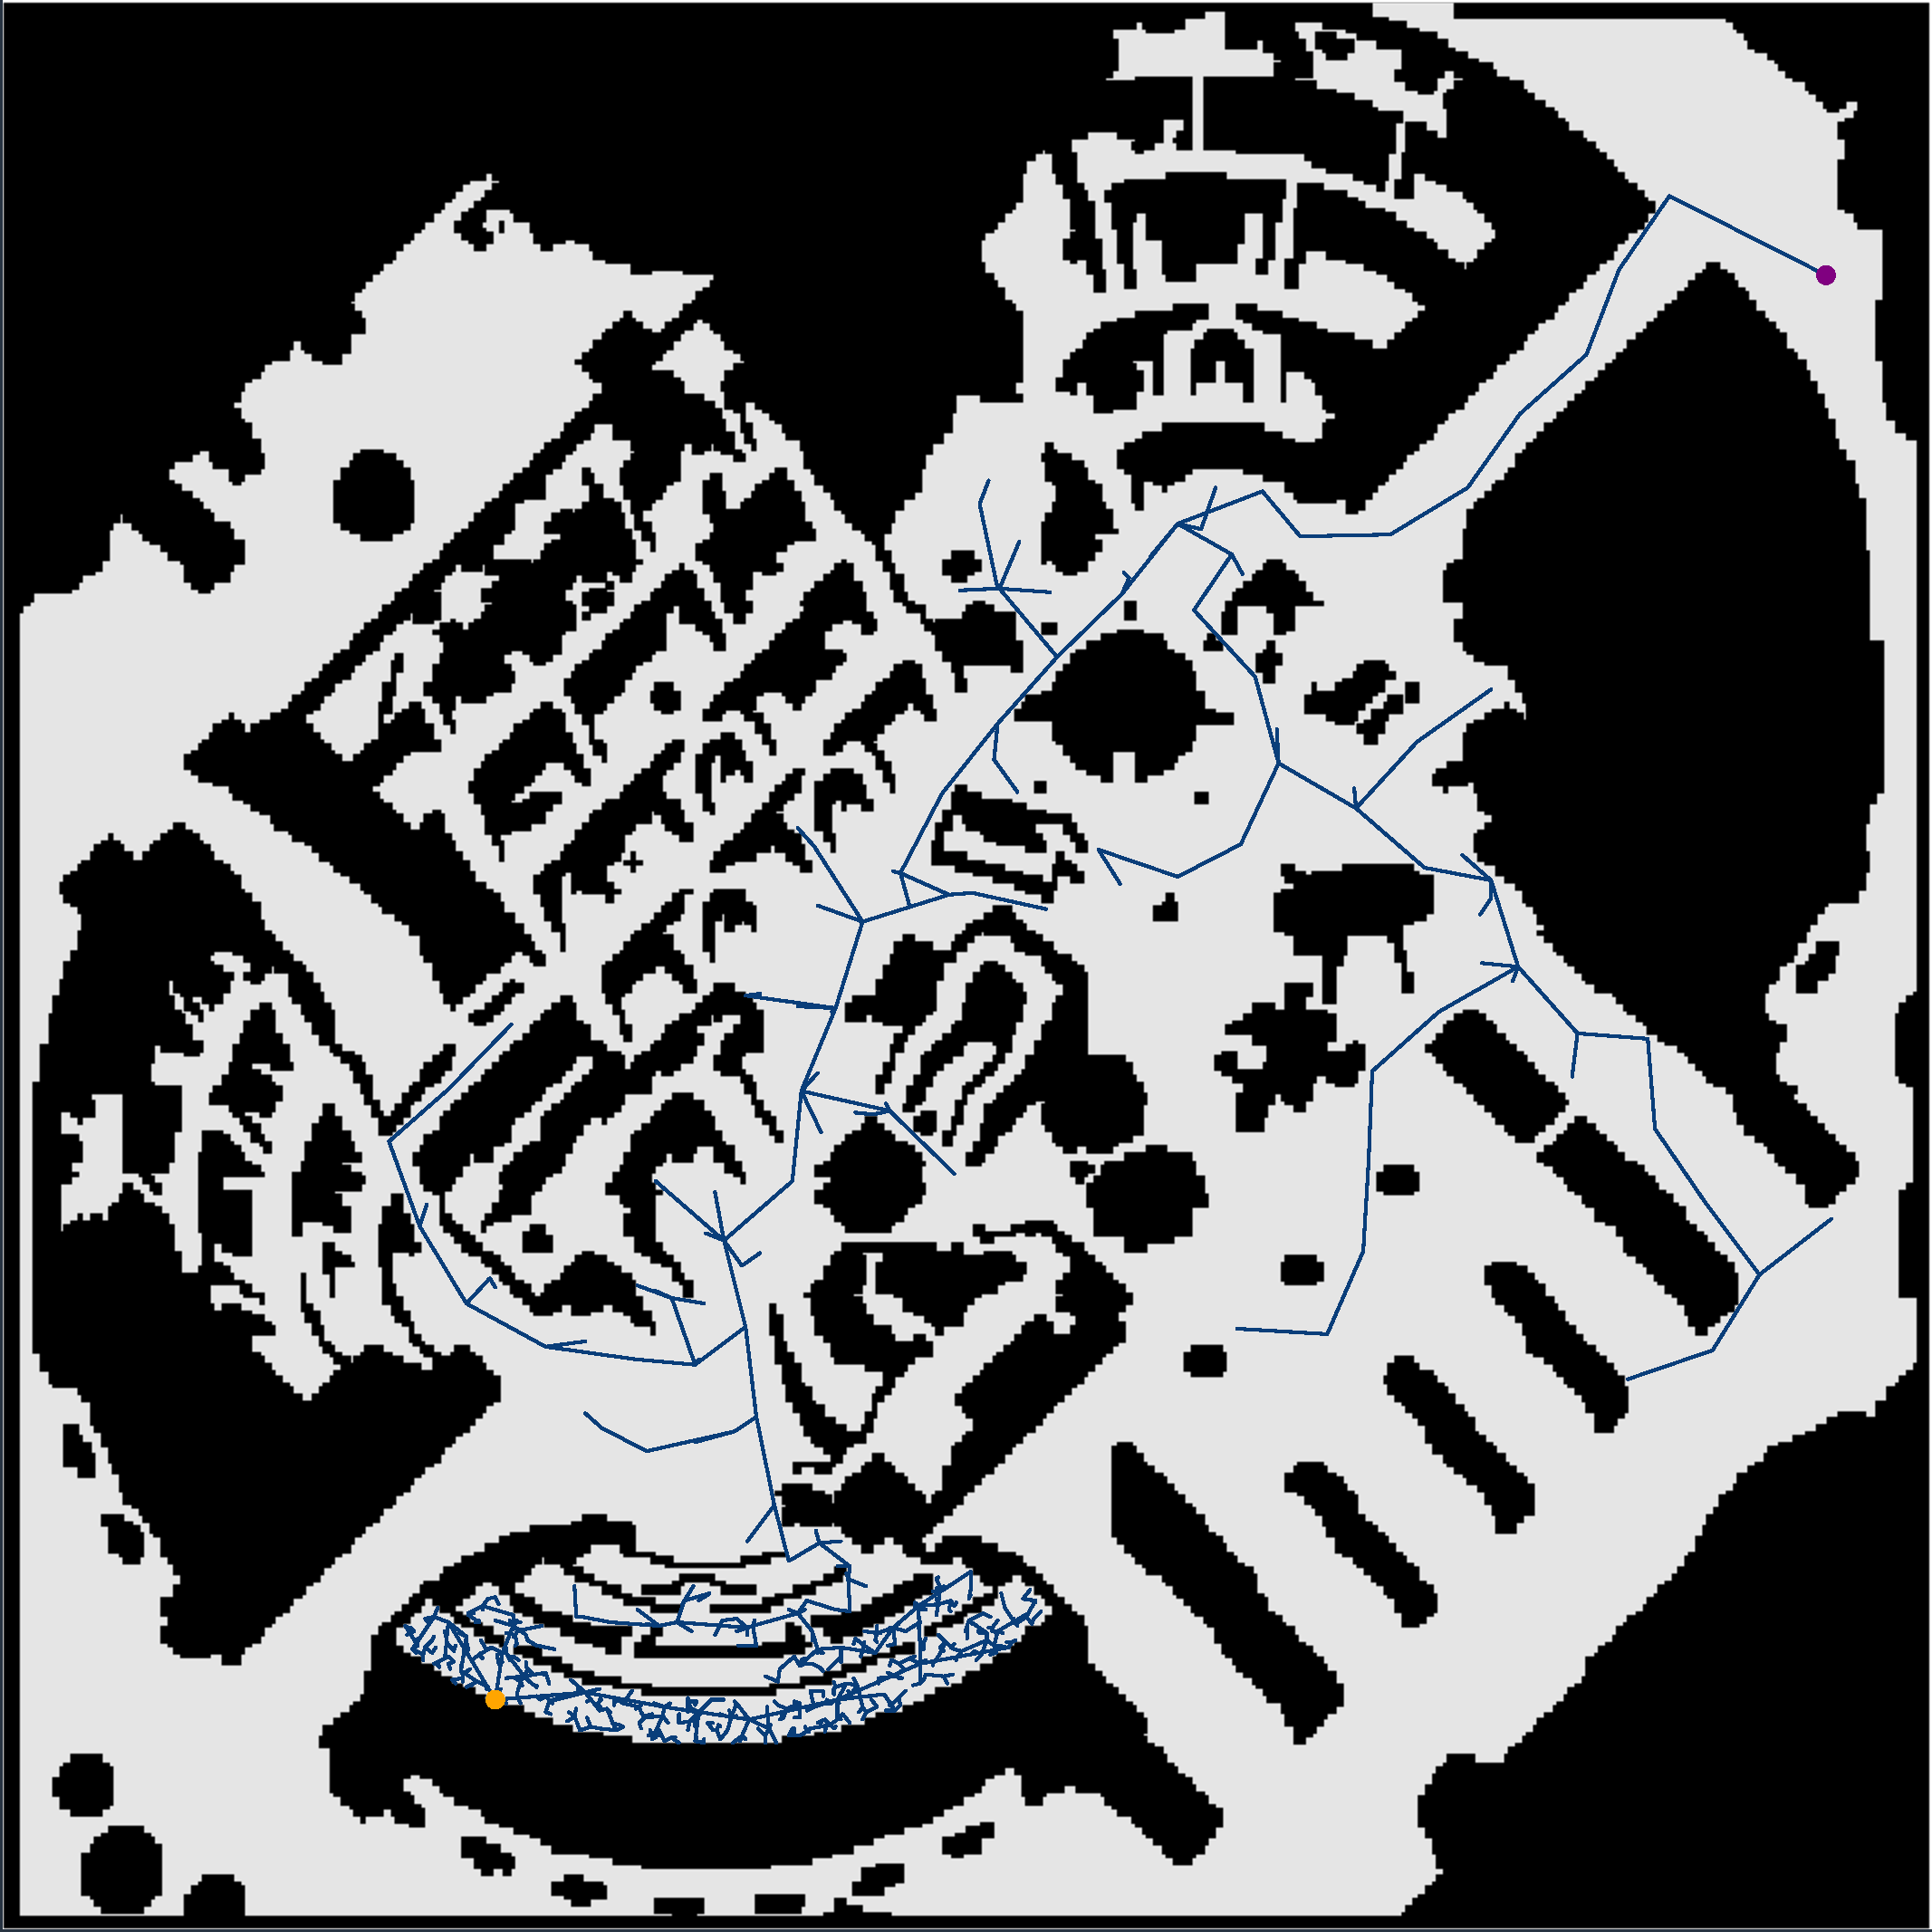
\includegraphics[width=1.0\linewidth, keepaspectratio]{figures/baldurs_rrt_one_off.pdf}
      \end{column}
      \begin{column}{.5\linewidth}
          {\Huge Path Planning}
          \begin{vfilleditems}
              \item {\Large Graph-based}
              \vspace{1em}
              \item {\Large Sample-based \Medium (left)}
              \vspace{1em}
              \item {\color{grey} {\Large Dynamic}}
          \end{vfilleditems}
          \vspace{1em}
          {\color{grey} {\Large Symbolic Regression}}
          \vspace{1em}
          {\color{grey} {\Large Neural Arch. Search}}
      \end{column}
  \end{columns}
\end{frame}

\begin{frame}[plain]{Graph-based search (Paris)}
    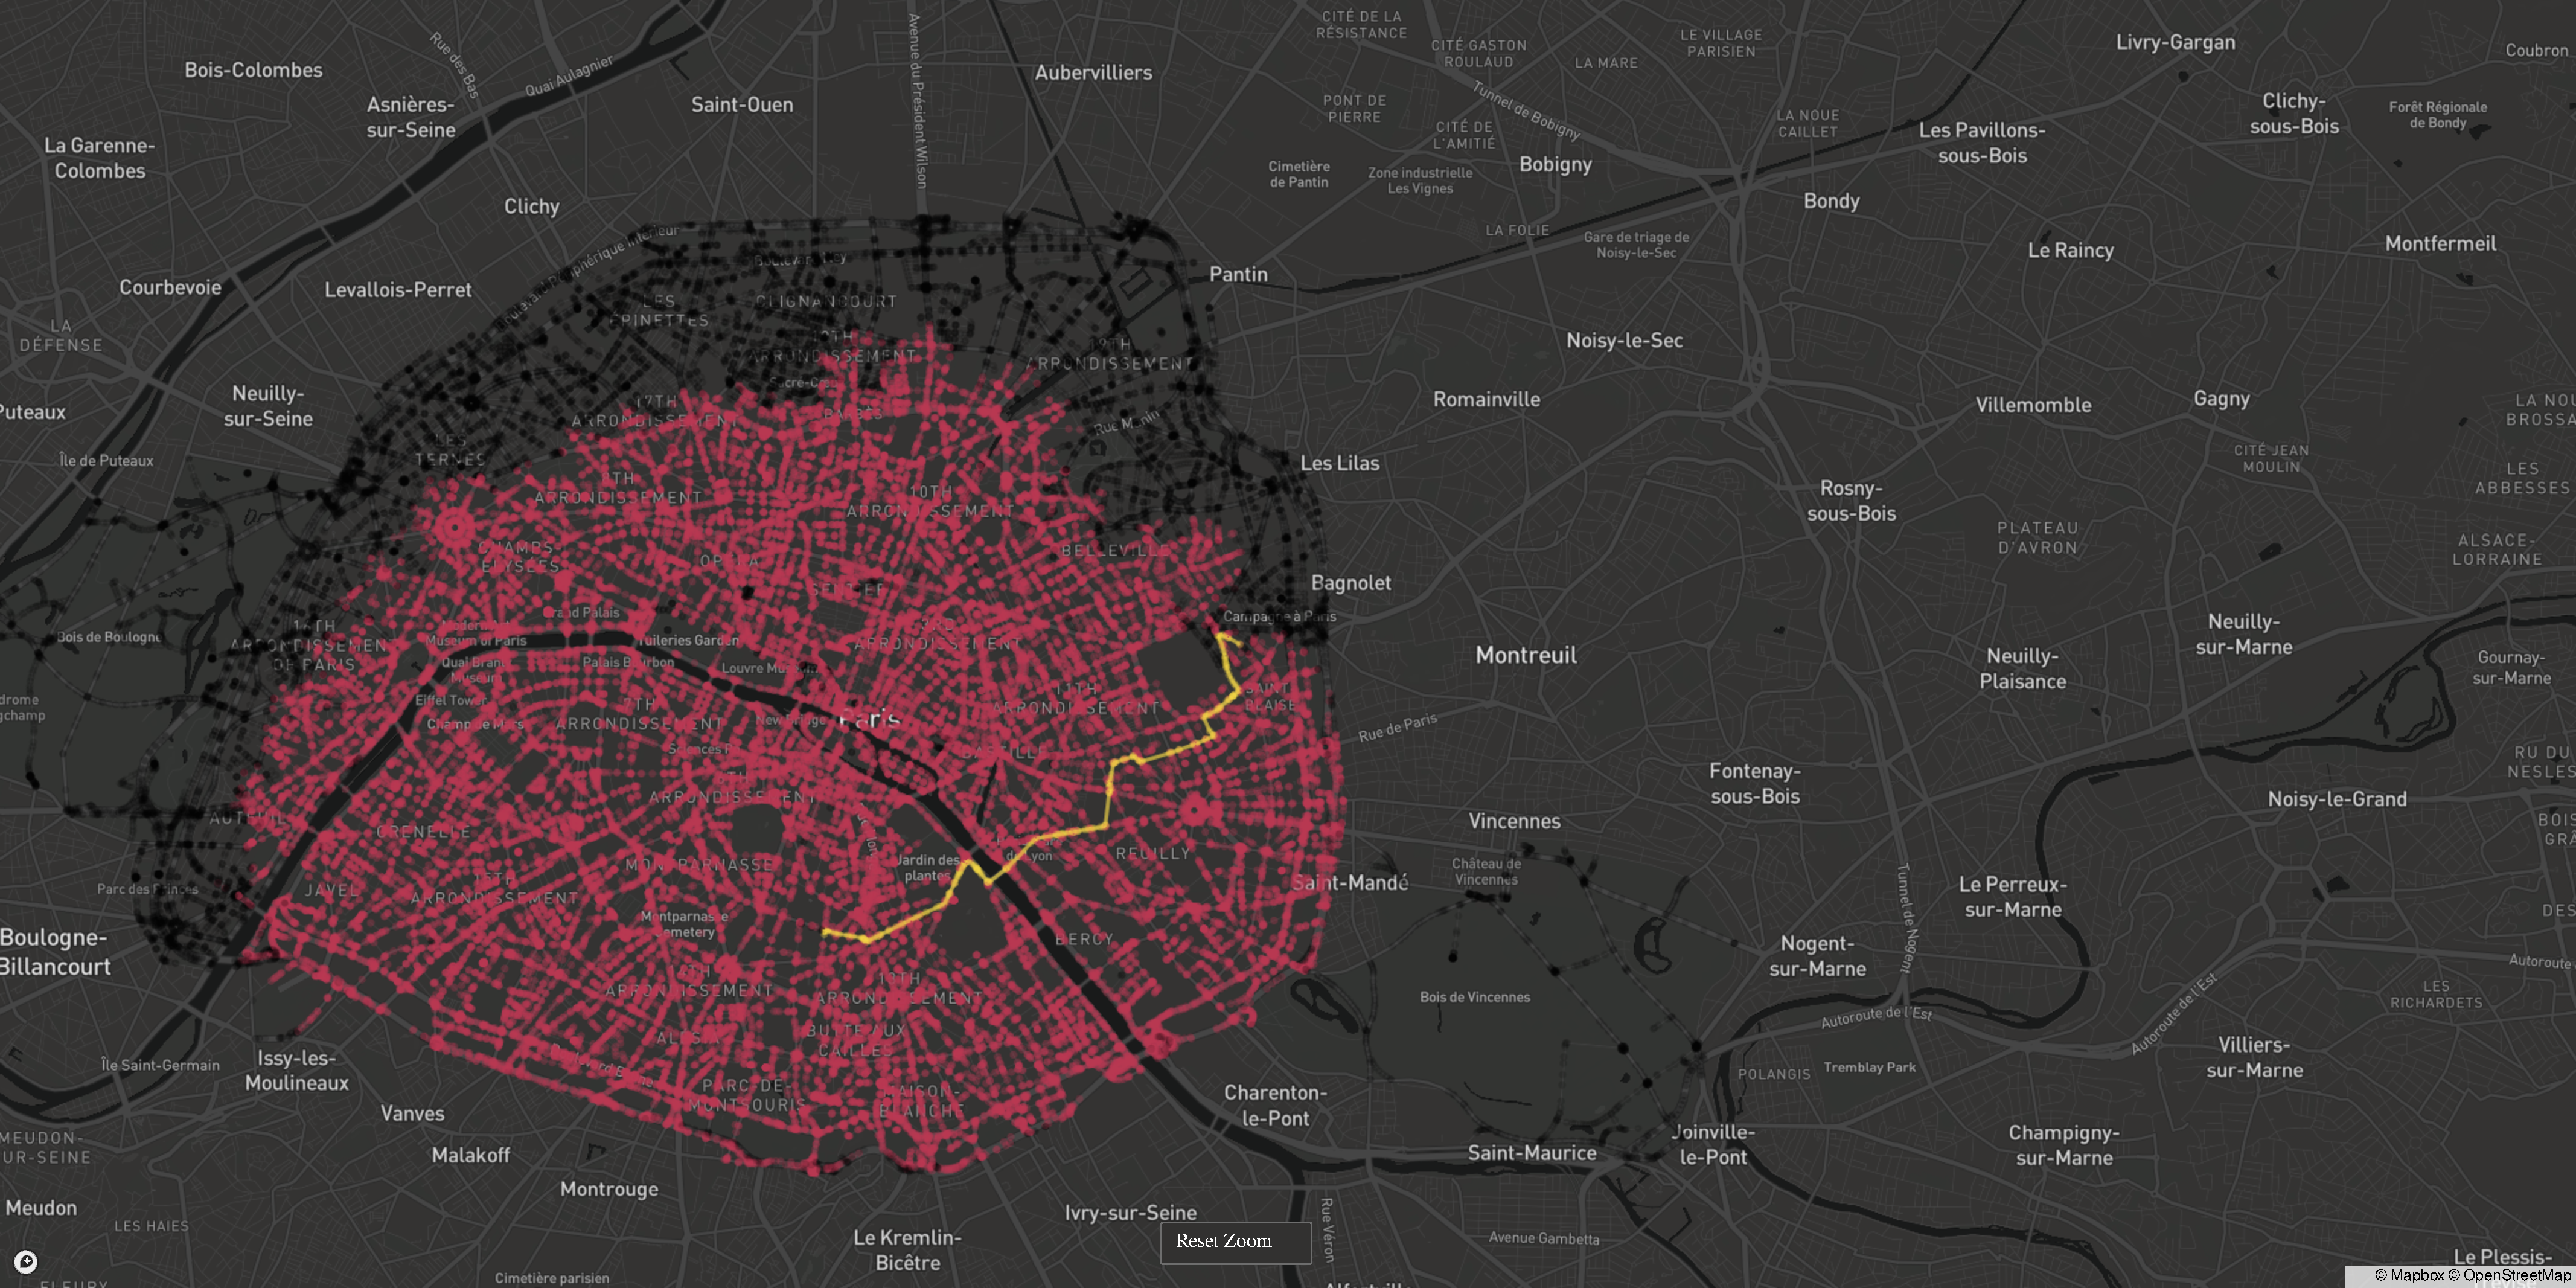
\includegraphics[height=0.9\textheight, keepaspectratio]{figures/paris_graph_based.pdf}
\end{frame}

\begin{frame}[plain]{Graph-based search (New York)}
    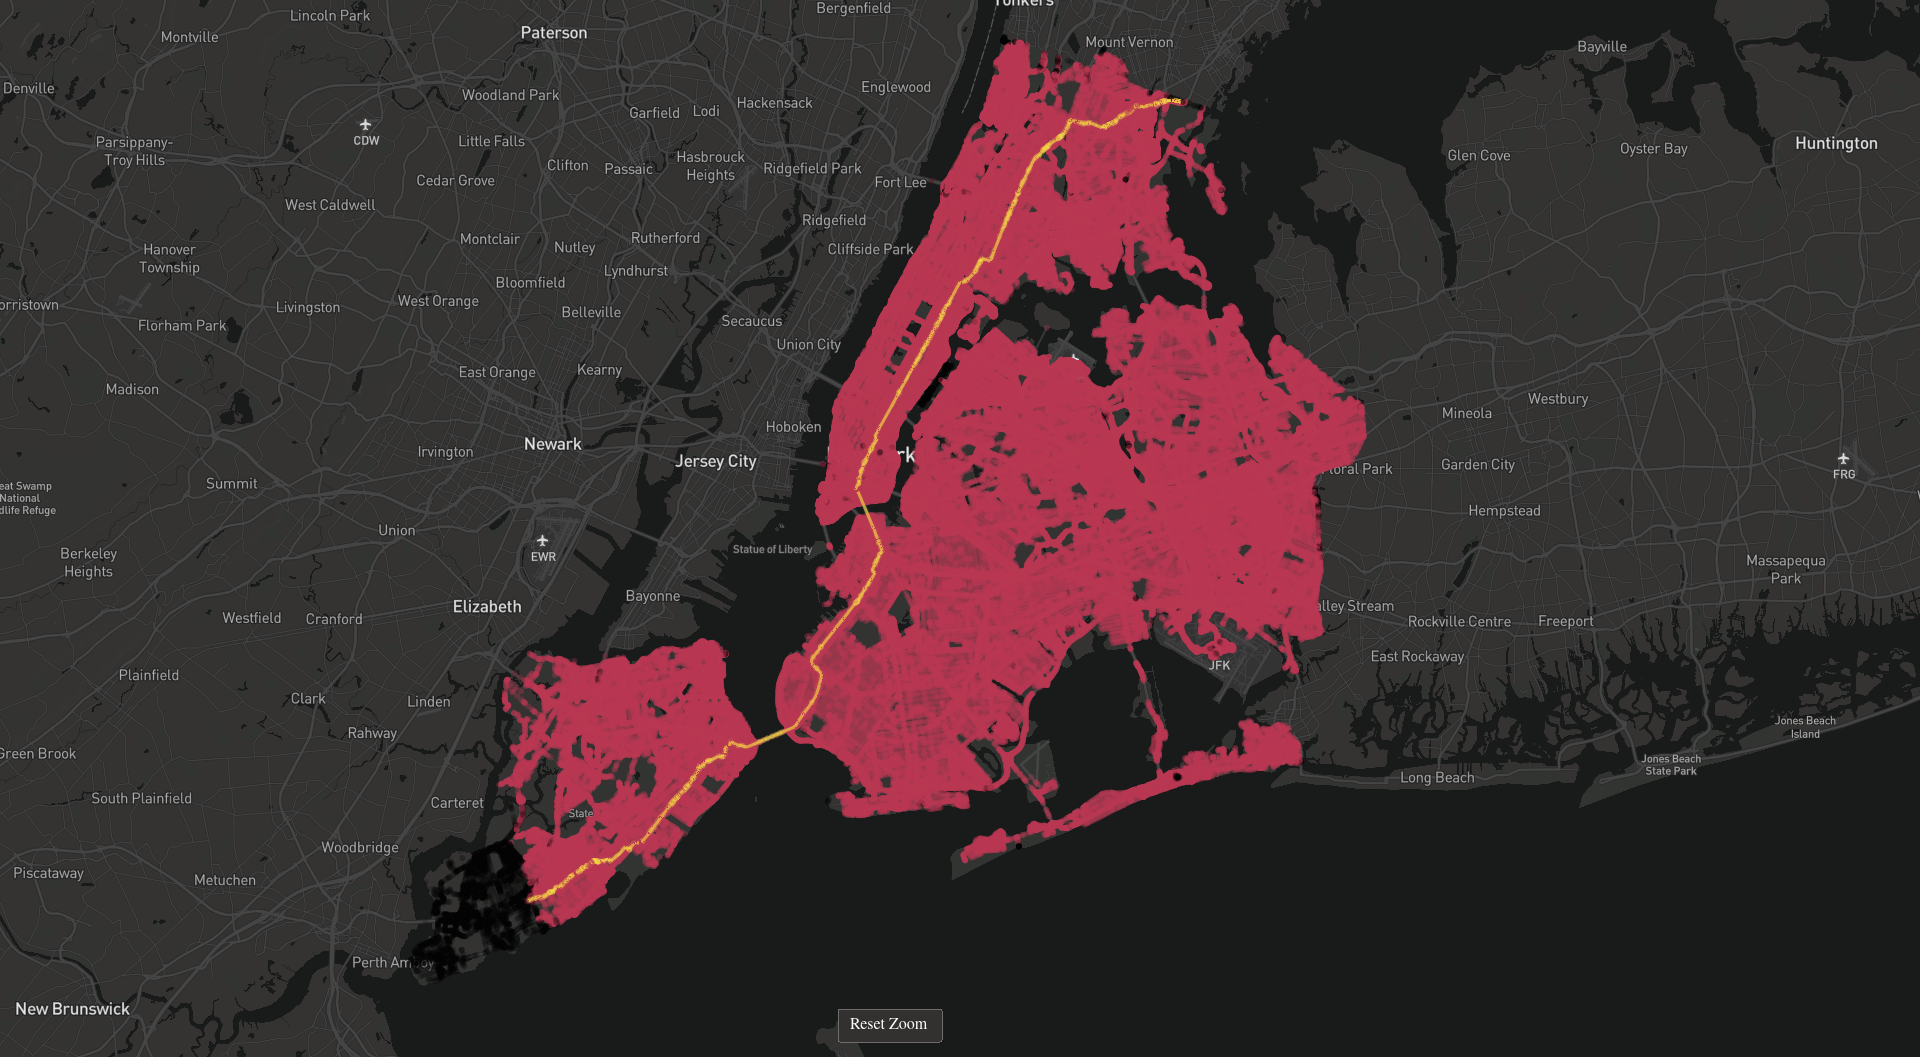
\includegraphics[height=0.9\textheight, keepaspectratio]{figures/ny_graph_based.png}
\end{frame}

\begin{frame}{Maps {\Medium \color{white}( \cite{sturtevant2012benchmarks})}}
    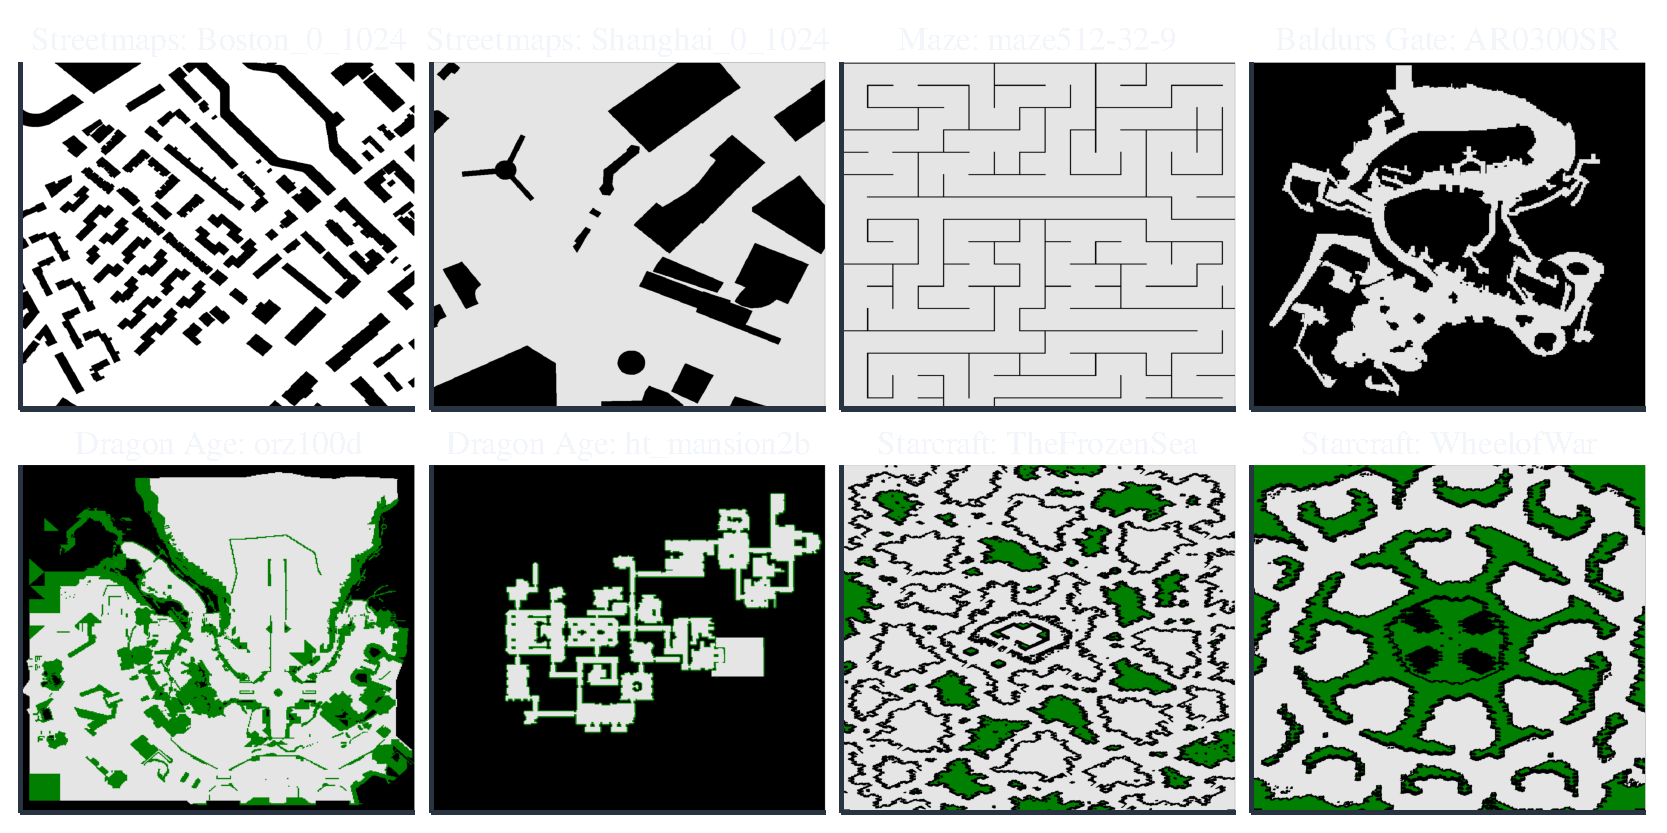
\includegraphics[width=1.0\linewidth, keepaspectratio]{figures/show_maps.pdf}
\end{frame}

\begin{frame}{Maps (Overview)}
    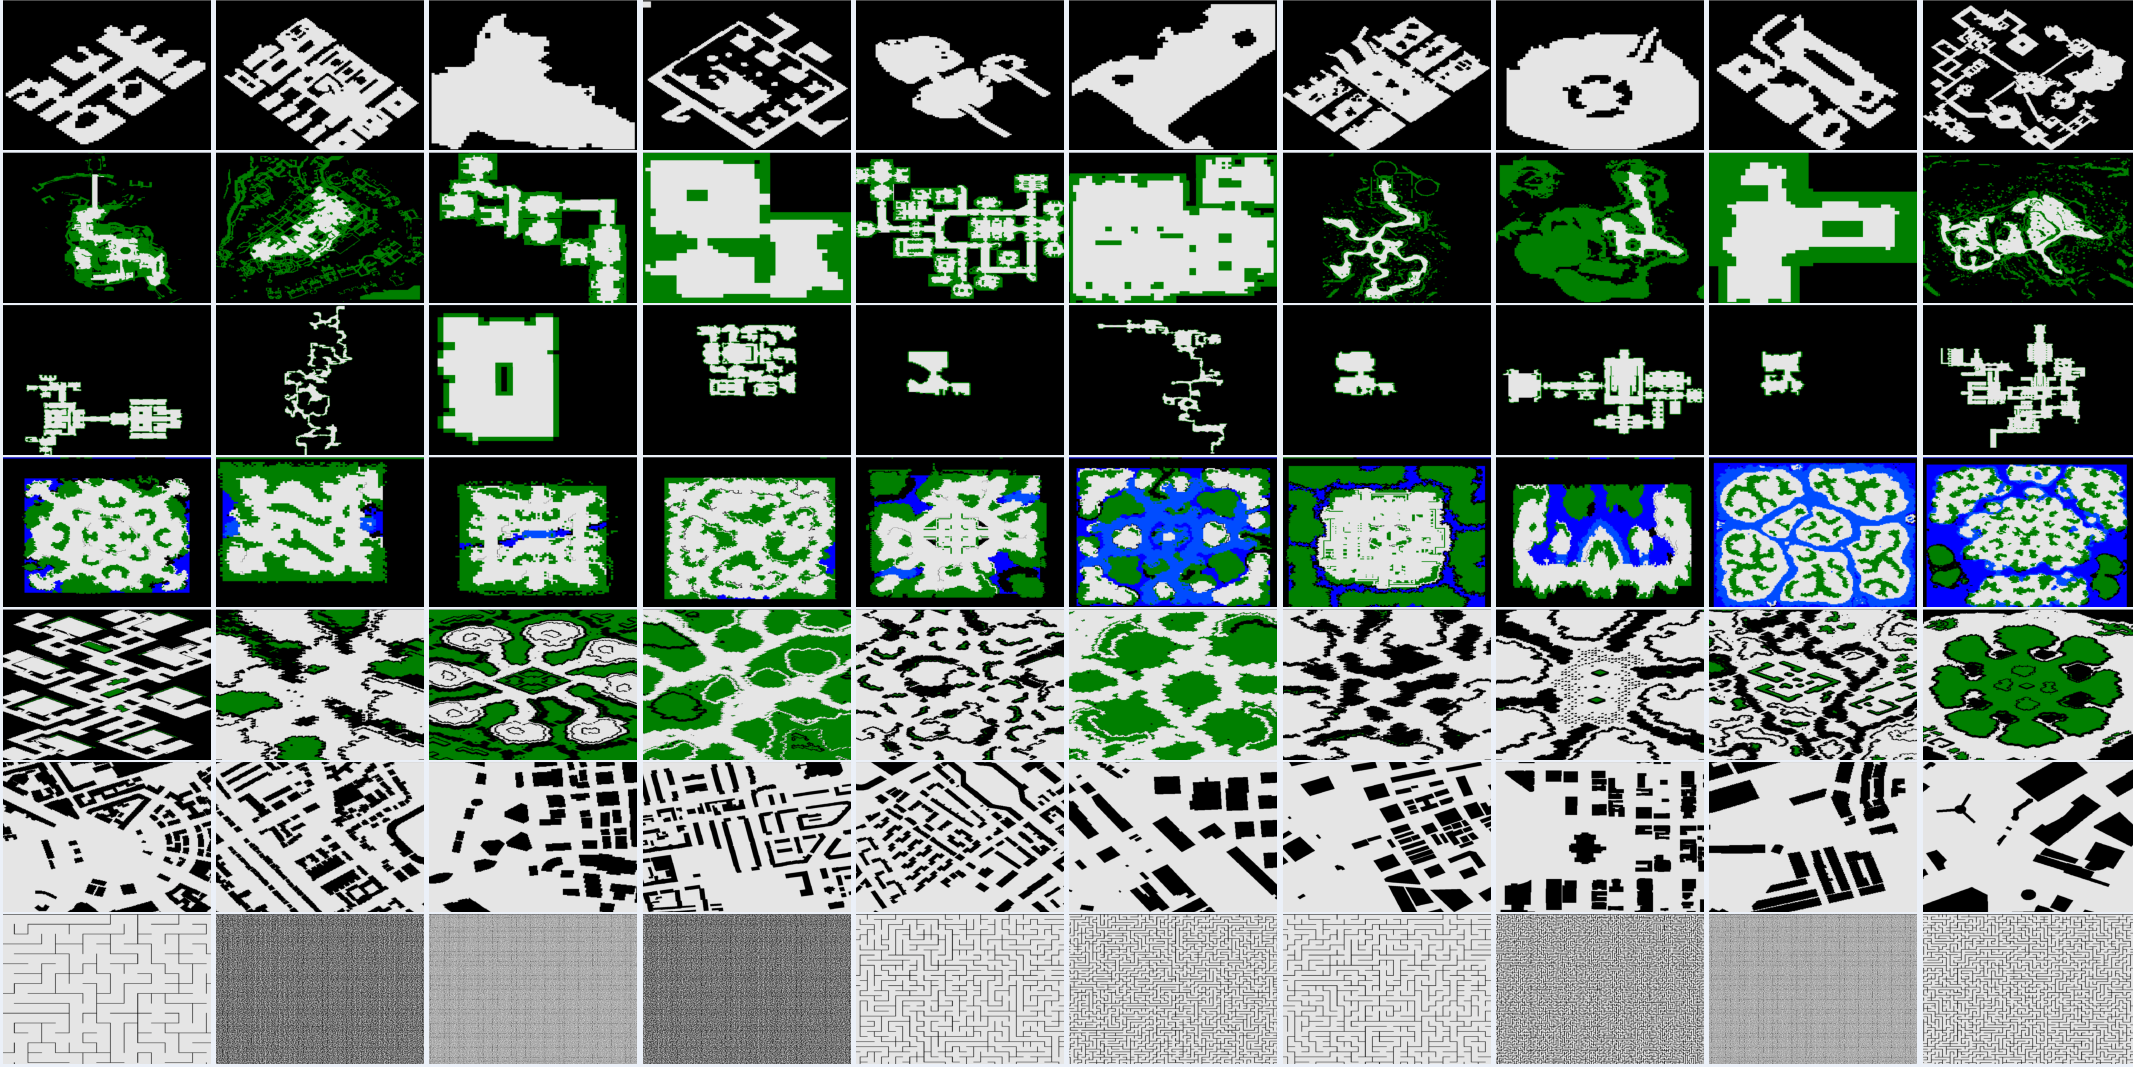
\includegraphics[width=1.0\linewidth, keepaspectratio]{figures/show_maps_overview.pdf}
\end{frame}

\begin{frame}{Outcomes}
    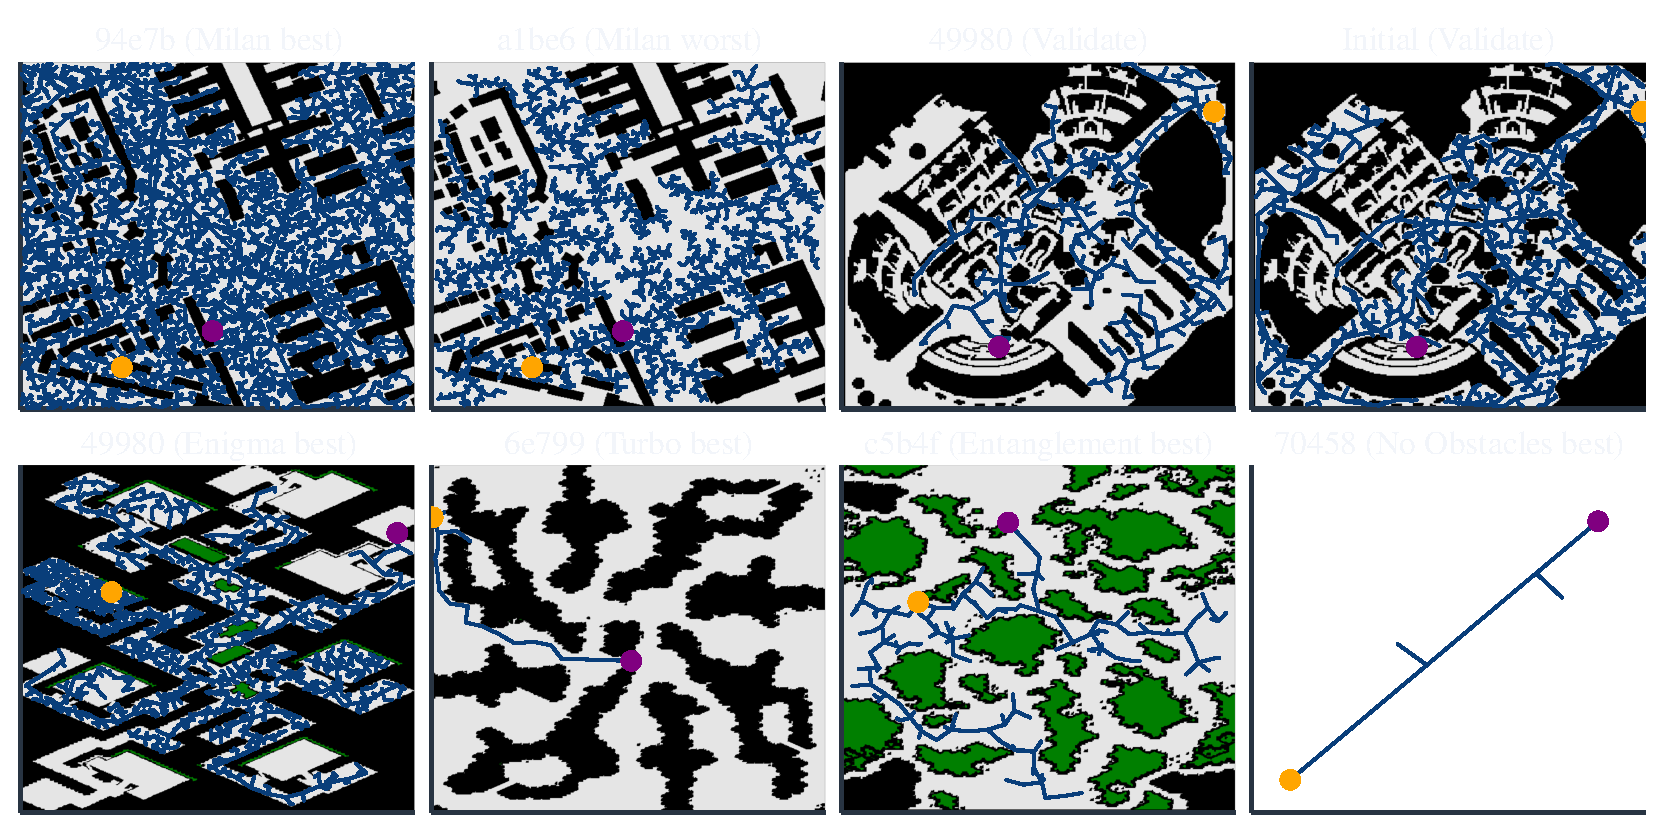
\includegraphics[width=1.0\linewidth, keepaspectratio]{figures/learned.pdf}
\end{frame}


\begin{frame}[plain]{Thesis}
    \begin{vfilleditems}
      \item {\Huge Evolution is powerful}
        \begin{itemize}
          \item {\Medium Responsible for Earth's diverse, adaptive life}
          \item {\Medium \color{pureminimalistic@text@red} Evolved intelligence}
        \end{itemize}
      \item {\Huge Learned representation matters}
    \end{vfilleditems}
\end{frame}

\begin{frame}{Research Questions}
  \begin{vfilleditems}
    \item {\Huge Is Genetic Programming Competitive in 2021? {\color{pureminimalistic@text@red} Yes.}}
    % TODO: Answer each at high level
    {\color{grey}
    \item {\Huge Is crossover necessary?}
    \item {\Huge What is the role of latent code?}
    \item {\Huge How should code be mutated?}
    \item {\Huge How hard is a problem?}
    }
  \end{vfilleditems}
\end{frame}

\begin{frame}{Research Questions}
  \begin{vfilleditems}
    \item {\Huge Role of program representation?}
    \item {\Huge Role of scale and compute efficiency?}
    \item {\Huge How should code be mutated?}
    \item {\Huge How hard is a problem?}
  \end{vfilleditems}
\end{frame}

\begin{frame}[plain]{On Bio-inspiration}
    \begin{vfilleditems}
      \item {\Medium Genetic programming is at best an analogy}
      \item {\Medium Many bio-inspired algorithms are simply inspired}
    \end{vfilleditems}
\end{frame}

\begin{frame}
    \item {\Huge Engineering has a huge role in ML algorithm success}
    \item {\Huge So: Genetic Programming}
      \begin{itemize}
        \item {\Medium Models environments naturally}
        \item {\Medium Highly interpretable}
      \end{itemize}
\end{frame}


\begin{frame}{History}
  \begin{columns}[T]
      \begin{column}{.5\linewidth}
          \begin{vfilleditems}
              \item {\Large Genetic algorithms first invented in 1960s}
              \vspace{1em}
              \item {\Large Recently surfaced for neural architecture meta-learning}
          \end{vfilleditems}
      \end{column}
      \begin{column}{.5\linewidth}
          \begin{vfilleditems}
              
\includegraphics[width=6cm, keepaspectratio]{figures/genetic.jpg}
          \end{vfilleditems}
      \end{column}
  \end{columns}
\end{frame}

% \item {\Huge \color{pureminimalistic@text@red} No Free Lunch}
%   \begin{itemize}
%     \item {\Medium Across all domains, algorithms are equal}
%   \end{itemize}

\appendix % do not count the following slides for the total number
\section*{Backup Slides}
\begin{frame}[plain, noframenumbering]
  \centering
  \vfill
  {\fontsize{40}{50}\selectfont Questions?}
  \vfill
\end{frame}

\begin{frame}[plain, noframenumbering]
  \centering
  \printbibliography
\end{frame}

\end{document}